% ==========================================================
\clearpage
\pagebreak
\justifying
\renewcommand{\thesection}{E \arabic{section}}

\titleformat{\section}{\normalfont\LARGE\bfseries\color{black}}{\thesection}{10pt}{\LARGE}
\section{Appendix-E5 Research Implementation Plan}\label{sec:App5-Research-Implementation-Plan}

%============================================================
\subsection{App5-PhD Proposal Document Preparation}
\begin{figure}[htbp]
	\begin{center}
		\frame{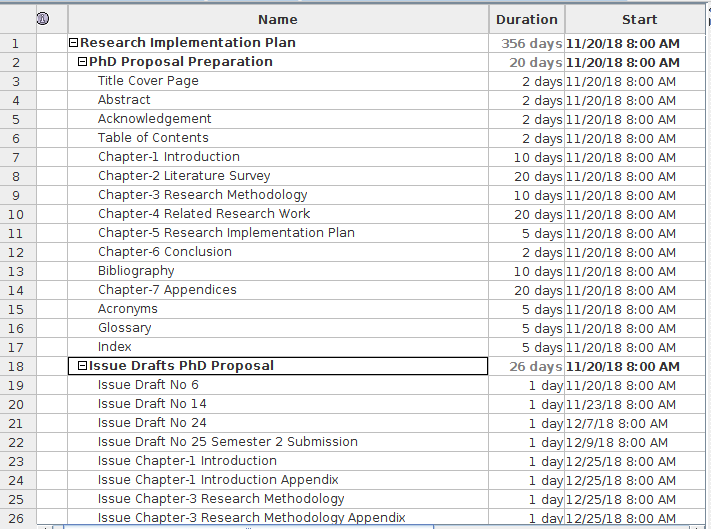
\includegraphics[width=1.00\textwidth]{./07-images/img-Ch5App/01-Research-Implementation-Plan.png}}
		\caption{App5-PhD Proposal Document Preparation}
		\label{fig:App5-01-Research-Implementation-Plan.png}
	\end{center}
\end{figure}

Note that the contents of a proposal document do not include the chapter on implementation design and the chapter on results and discussion, which are both required for a thesis document.

	
\pagebreak	
\subsection{App5-Procurement of Long Lead Items and Project Setup}
\begin{figure}[htbp]
	\begin{center}
		\frame{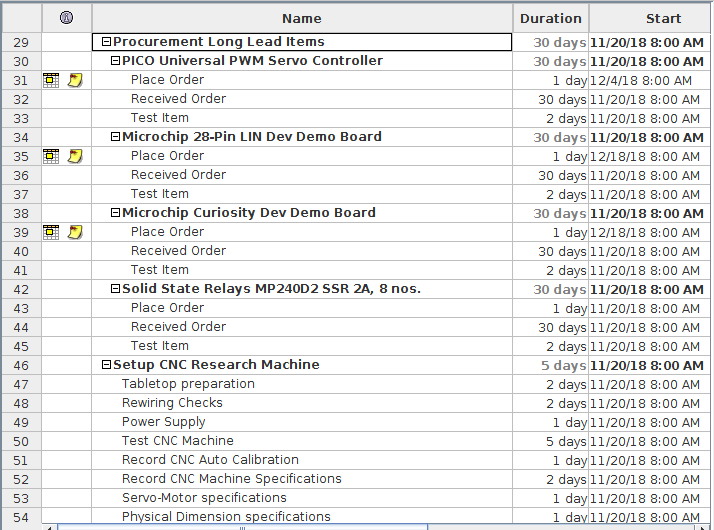
\includegraphics[width=1.00\textwidth]{./07-images/img-Ch5App/02-Research-Implementation-Plan.png}}
		\caption{App5-Procurement of Long Lead Items and Project Setup}
		\label{fig:App5-02-Research-Implementation-Plan.png}
	\end{center}
\end{figure}

The long lead items above are hardware resources that must be procured for the project.

\pagebreak
\subsection{App5-Computer 64bit Resources and Software Installations}
\begin{figure}[htbp]
	\begin{center}
		\frame{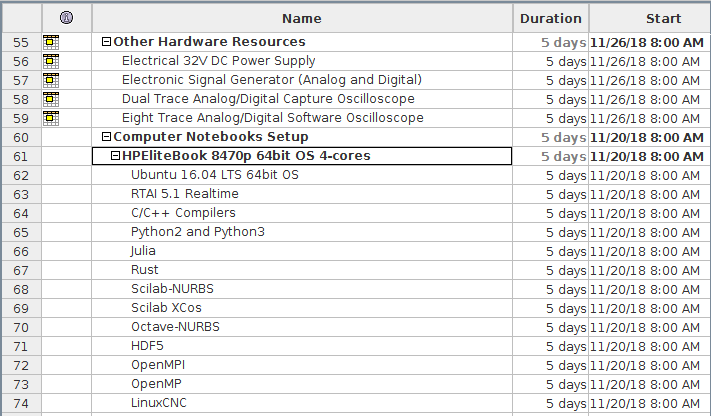
\includegraphics[width=1.00\textwidth]{./07-images/img-Ch5App/03-Research-Implementation-Plan.png}}
		\caption{App5-Computer 64bit Resources and Software Installations}
		\label{fig:App5-03-Research-Implementation-Plan.png}
	\end{center}
\end{figure}

We will be implementing the CNC Control software on both 64bit and 32bit systems. The Linux kernel for the 64bit system is of version 4.X, while that for the 32bit system is of version 3.X. The Realtime RTAI library for the 64bit system is of version 5.1, while that for the 32bit system is version 2.7.  
\vspace{0.5cm}

The above tasks in the figure identify the 64bit hardware resources and their associated software that are required for the project.

\pagebreak
\subsection{App5-Computer 32bit Resources and Software Installations}
\begin{figure}[htbp]
	\begin{center}
		\frame{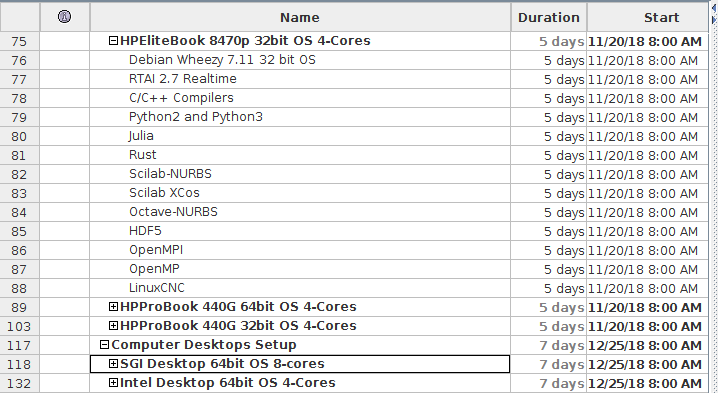
\includegraphics[width=1.00\textwidth]{./07-images/img-Ch5App/04-Research-Implementation-Plan.png}}
		\caption{App5-Computer 32bit Resources and Software Installations}
		\label{fig:App5-04-Research-Implementation-Plan.png}
	\end{center}
\end{figure}

We will be implementing the CNC Control software on four(4) different computer hardware configurations (number of CPU cores, memory speeds, hard disk speeds, etc) for the purposes of performance comparisons. The multi-core feature of the computers is for true parallel computation design. The different computers are as follows:

\begin{enumerate}
	\item Notebook HP EliteBook 8470p, 4-cores, installed with both 64bit and 32bit Linux operating systems.   
	
	\item Notebook HP ProBook 440G, 4-cores, installed with both 64bit and 32bit Linux operating systems.
	
	\item Desktop SGI, 8-cores, installed with only 64bit Linux operating system. Does not accept 32bit OS.
	
	\item Desktop Intel, 4-cores, installed with both 64bit and 32bit Linux operating systems.
\end{enumerate}

The above tasks in the figure identify the 32bit hardware resources and their associated software that are required for the project.

\pagebreak
\subsection{App5-UseCase Design and Software Architecture Design}\label{sec:App5-UseCase Design}
\begin{figure}[htbp]
	\begin{center}
		\frame{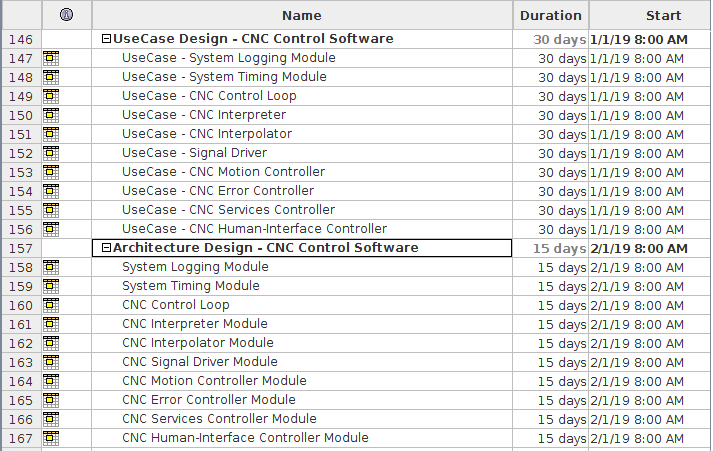
\includegraphics[width=1.00\textwidth]{./07-images/img-Ch5App/05-Research-Implementation-Plan.png}}
		\caption{App5-UseCase Design and Software Architecture Design}
		\label{fig:App5-05-Research-Implementation-Plan.png}
	\end{center}
\end{figure}


\pagebreak	
\subsection{App5-Process and Data Flow Design for the Control Loop}\label{sec:App5-Process-Flow Design}
\begin{figure}[htbp]
	\begin{center}
		\frame{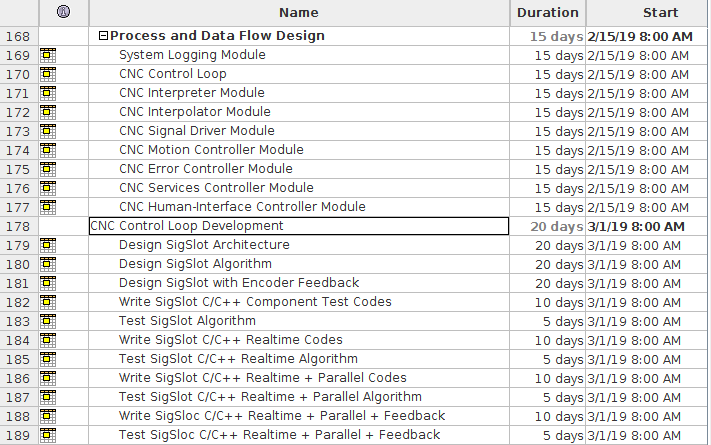
\includegraphics[width=1.00\textwidth]{./07-images/img-Ch5App/06-Research-Implementation-Plan.png}}
		\caption{App5-Process and Data Flow Design for the Control Loop}
		\label{fig:App5-06-Research-Implementation-Plan.png}
	\end{center}
\end{figure}

\pagebreak
\subsection{App5-Test-Case Based Design in Software Construction}
\begin{figure}[htbp]
	\begin{center}
		\frame{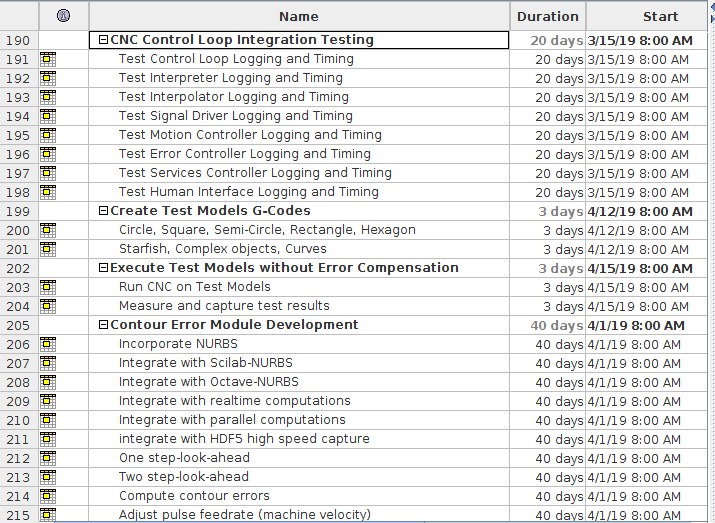
\includegraphics[width=1.00\textwidth]{./07-images/img-Ch5App/07-Research-Implementation-Plan.png}}
		\caption{App5-Test-Case Based Design in Software Construction}
		\label{fig:App5-07-Research-Implementation-Plan.png}
	\end{center}
\end{figure}

\pagebreak
\subsection{App5-Completion Testing, Publication Plan and Project Closing}
\begin{figure}[htbp]
	\begin{center}
		\frame{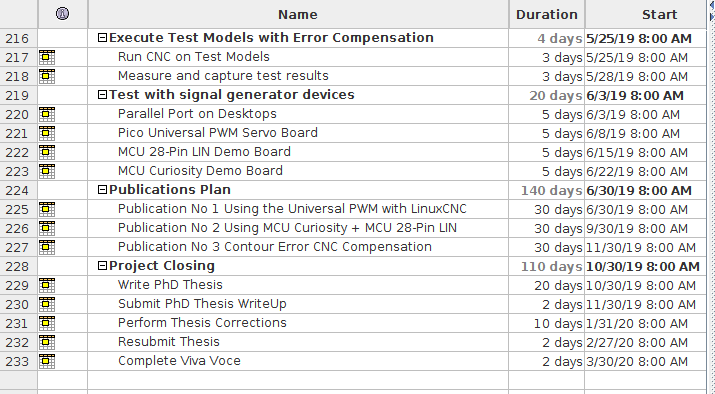
\includegraphics[width=1.00\textwidth]{./07-images/img-Ch5App/08-Research-Implementation-Plan.png}}
		\caption{App5-Completion Testing, Publication Plan and Project Closing}
		\label{fig:App5-08-Research-Implementation-Plan.png}
	\end{center}
\end{figure}

% ==========================================================
% ==========================================================
\clearpage
\begin{landscape}
\subsection{App5-Computer Notebook Specifications}
	
\begin{table}[ht]
\begin{center}
\caption{App5-Computer Notebook Specifications}		
\label{table:App5-Computer Notebook Specifications}	
	
\begin{tabular}{ |p{0.5cm}|p{5.0cm}|p{9.0cm}|p{9.0cm}|}
	\rowcolor{gray!10}			
	\hline \multicolumn{4}{|c|}{\textbf{Computer Notebook Specifications}} \\ [1.0ex]
	\rowcolor{gray!10}
	\hline \textbf{No} & \textbf{Specifications}    & \textbf{Hewlett Packard EliteBook 8470p} & \textbf{Hewlett Packard ProBook 440G}\\ 

	\hline 1 & Name of Student    & Wan Ruslan bin W Yusoff & hello\\ 
	\hline 2 & Student ID         &  aaa & Hello\\ 
	\hline 3 & National Reg. ID   & bbb  & Hello\\ 
	\hline 4 & Faculty            & ccc  & Hello\\ 

	\hline
\end{tabular}
\end{center}
\end{table}  
	
	
\end{landscape}
% ==========================================================
% ==========================================================
\clearpage
\begin{landscape}
\subsection{App5-Computer Desktop Specifications}
	
	\begin{table}[ht]
		\begin{center}
			\caption{App5-Computer Desktop Specifications}		
			\label{table:App5-Computer Desktop Specifications}	
			
			\begin{tabular}{ |p{0.5cm}|p{5.0cm}|p{9.0cm}|p{9.0cm}|}
				\rowcolor{gray!10}			
				\hline \multicolumn{4}{|c|}{\textbf{Computer Desktop Specifications}} \\ [1.0ex]
				\rowcolor{gray!10}
				\hline \textbf{No} & \textbf{Specifications}  & \textbf{WRY Intel Desktop} & \textbf{WRY SGI Desktop}\\ 
				
				\hline 1 & Name of Student    & Wan Ruslan bin W Yusoff & hello\\ 
				\hline 2 & Student ID         &  aaa & Hello\\ 
				\hline 3 & National Reg. ID   & bbb  & Hello\\ 
				\hline 4 & Faculty            & ccc  & Hello\\ 
				
				\hline
			\end{tabular}
		\end{center}
	\end{table}  
	
	
\end{landscape}
% ==========================================================
% ==========================================================
\clearpage
\begin{landscape}
\subsection{App5-Pulse Generator Interface Boards}
	
	\begin{table}[ht]
		\begin{center}
			\caption{App5-Pulse Generator Interface Boards}		
			\label{table:App5-Pulse Generator Interface Boards}	
			
			\begin{tabular}{ |p{0.5cm}|p{5.0cm}|p{6.0cm}|p{6.0cm}|p{6.0cm}|}
				\rowcolor{gray!10}			
				\hline \multicolumn{5}{|c|}{\textbf{Pulse Generator Interface Boards}} \\ [1.0ex]
				\rowcolor{gray!10}
				\hline \textbf{No} & \textbf{Specifications}    & \textbf{Pico Universal PWM Servo Controller Board} & \textbf{MCU Microchip 28-Pin LIN Development Board} & \textbf{MCU Microchip Curiosity Development Board}\\ 
				
				\hline 1 & Name of Student    & Wan Ruslan bin W Yusoff & hello & Hello\\ 
				\hline 2 & Student ID         &  aaa & Hello & hello\\ 
				\hline 3 & National Reg. ID   & bbb  & Hello & Hello \\ 
				\hline 4 & Faculty            & ccc  & Hello & Hello\\ 
				
				\hline
			\end{tabular}
		\end{center}
	\end{table}  
	
	
\end{landscape}
% ==========================================================
% ==========================================================
\clearpage
\begin{landscape}
\subsection{App5-Software Programming Language Features}

	
	\begin{table}[ht]
		\begin{center}
			\caption{App5-Software Programming Language Features}		
			\label{table:App5-Software Programming Language Features}	
			
			\begin{tabular}{ |p{0.5cm}|p{5.0cm}|p{9.0cm}|p{9.0cm}|}
				\rowcolor{gray!10}			
				\hline \multicolumn{4}{|c|}{\textbf{Software Programming Language Features}} \\ [1.0ex]
				\rowcolor{gray!10}
				\hline \textbf{No} & \textbf{Specifications}    & \textbf{Hewlett Packard EliteBook 8470p} & \textbf{Hewlett Packard ProBook 440G}\\ 
				
				\hline 1 & Name of Student    & Wan Ruslan bin W Yusoff & hello\\ 
				\hline 2 & Student ID         &  aaa & Hello\\ 
				\hline 3 & National Reg. ID   & bbb  & Hello\\ 
				\hline 4 & Faculty            & ccc  & Hello\\ 
				
				\hline
			\end{tabular}
		\end{center}
	\end{table}  
	
	
\end{landscape}
% ==========================================================
% ==========================================================
\clearpage
\begin{landscape}
\subsection{App5-Software Programming Paradigms}
	
	\begin{table}[ht]
		\begin{center}
			\caption{App5-Software Programming Paradigms}		
			\label{table:App5-Software Programming Paradigms}	
			
			\begin{tabular}{ |p{0.5cm}|p{5.0cm}|p{9.0cm}|p{9.0cm}|}
				\rowcolor{gray!10}			
				\hline \multicolumn{4}{|c|}{\textbf{Software Programming Paradigms}} \\ [1.0ex]
				\rowcolor{gray!10}
				\hline \textbf{No} & \textbf{Specifications}    & \textbf{Hewlett Packard EliteBook 8470p} & \textbf{Hewlett Packard ProBook 440G}\\ 
				
				\hline 1 & Name of Student    & Wan Ruslan bin W Yusoff & hello\\ 
				\hline 2 & Student ID         &  aaa & Hello\\ 
				\hline 3 & National Reg. ID   & bbb  & Hello\\ 
				\hline 4 & Faculty            & ccc  & Hello\\ 
				
				\hline
			\end{tabular}
		\end{center}
	\end{table}  
	
\end{landscape}	
% ==========================================================
% ==========================================================
\clearpage
\begin{landscape}
	\subsection{App5-Scilab NURBS versus Octave NURBS packages}
	
	\begin{table}[ht]
		\begin{center}
			\caption{App5-Scilab NURBS versus Octave NURBS packages}		
			\label{tabl2:App5-Scilab NURBS versus Octave NURBS packages}	
			
			\begin{tabular}{ |p{0.5cm}|p{5.0cm}|p{9.0cm}|p{9.0cm}|}
				\rowcolor{gray!10}			
				\hline \multicolumn{4}{|c|}{\textbf{Scilab NURBS versus Octave NURBS packages}} \\ [1.0ex]
				\rowcolor{gray!10}
				\hline \textbf{No} & \textbf{Specifications}    & \textbf{Hewlett Packard EliteBook 8470p} & \textbf{Hewlett Packard ProBook 440G}\\ 
				
				\hline 1 & Name of Student    & Wan Ruslan bin W Yusoff & hello\\ 
				\hline 2 & Student ID         &  aaa & Hello\\ 
				\hline 3 & National Reg. ID   & bbb  & Hello\\ 
				\hline 4 & Faculty            & ccc  & Hello\\ 
				
				\hline
			\end{tabular}
		\end{center}
	\end{table}  
	
\end{landscape}
% ==========================================================
% ==========================================================
\clearpage
\begin{landscape}
	\subsection{App5-Python versus Julia programming languages}
	
	\begin{table}[ht]
		\begin{center}
			\caption{App5-Python versus Julia programming languages}		
			\label{tabl2:App5-Python versus Julia programming languages}	
			
			\begin{tabular}{ |p{0.5cm}|p{5.0cm}|p{9.0cm}|p{9.0cm}|}
				\rowcolor{gray!10}			
				\hline \multicolumn{4}{|c|}{\textbf{Python versus Julia programming languages}} \\ [1.0ex]
				\rowcolor{gray!10}
				\hline \textbf{No} & \textbf{Specifications}    & \textbf{Hewlett Packard EliteBook 8470p} & \textbf{Hewlett Packard ProBook 440G}\\ 
				
				\hline 1 & Name of Student    & Wan Ruslan bin W Yusoff & hello\\ 
				\hline 2 & Student ID         &  aaa & Hello\\ 
				\hline 3 & National Reg. ID   & bbb  & Hello\\ 
				\hline 4 & Faculty            & ccc  & Hello\\ 
				
				\hline
			\end{tabular}
		\end{center}
	\end{table}  
	
\end{landscape}
% ==========================================================
% ==========================================================
\clearpage
\begin{landscape}
	\subsection{App5-C/C++ versus Rust system programming languages}
	
	\begin{table}[ht]
		\begin{center}
			\caption{App5-C/C++ versus Rust system programming languages}		
			\label{tabl2:App5-C/C++ versus Rust system programming languages}	
			
			\begin{tabular}{ |p{0.5cm}|p{5.0cm}|p{9.0cm}|p{9.0cm}|}
				\rowcolor{gray!10}			
				\hline \multicolumn{4}{|c|}{\textbf{C/C++ versus Rust system programming languages}} \\ [1.0ex]
				\rowcolor{gray!10}
				\hline \textbf{No} & \textbf{Specifications}    & \textbf{Hewlett Packard EliteBook 8470p} & \textbf{Hewlett Packard ProBook 440G}\\ 
				
				\hline 1 & Name of Student    & Wan Ruslan bin W Yusoff & hello\\ 
				\hline 2 & Student ID         &  aaa & Hello\\ 
				\hline 3 & National Reg. ID   & bbb  & Hello\\ 
				\hline 4 & Faculty            & ccc  & Hello\\ 
				
				\hline
			\end{tabular}
		\end{center}
	\end{table}  
	
\end{landscape}
% ==========================================================
% ==========================================================
